\documentclass[10pt,letterpaper]{article}
\usepackage{geometry}
\geometry{letterpaper, portrait, margin=0.5in}
\usepackage[utf8]{inputenc}
\usepackage{amsmath}
\usepackage{amsfonts}
\usepackage{amssymb}
\usepackage{graphicx}
\usepackage{subcaption}
\usepackage{array}
\usepackage{hyperref}
\usepackage{adjustbox,lipsum}
\usepackage{gensymb}
\setlength{\parindent}{0pt}
\renewcommand\refname{References}

\begin{document}
\title{\scshape\LARGE University of Waterloo \vfill \huge\bfseries PHYS 474 Assignment 1 \vfill}
\author{Robert Burnet \\ rcburnet@uwaterloo.ca \\ 20465122 }
\maketitle

\newpage

\textbf{1.} a)
\begin{figure}[h!]
\center
\caption{Sorted Galaxies}\label{fig: Sorted Galaxies}
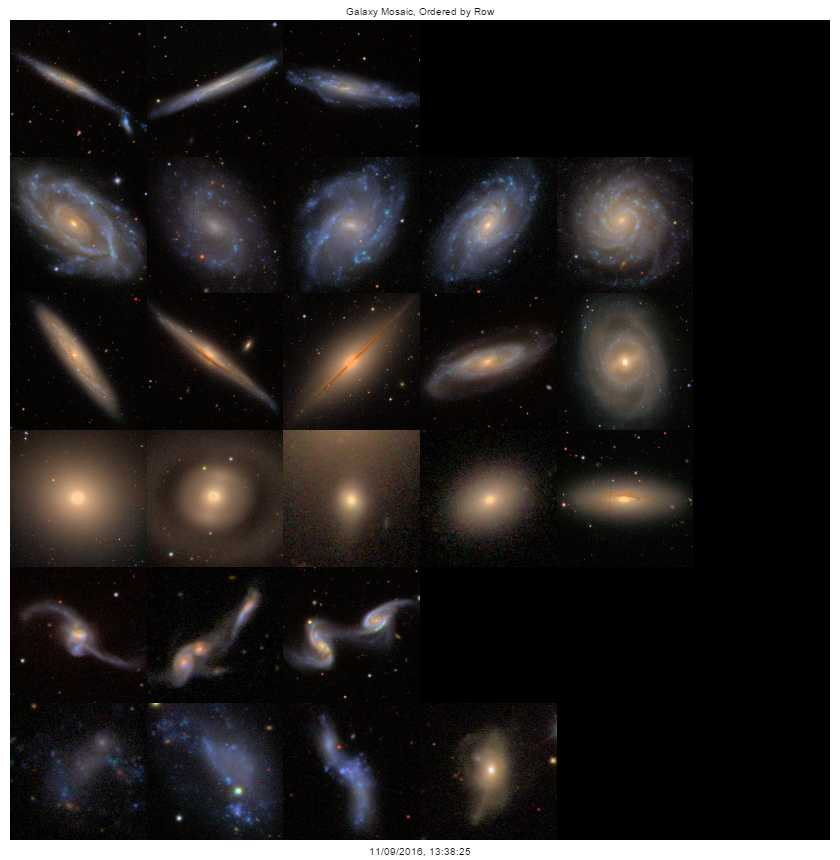
\includegraphics[scale=0.4]{figures/galaxy_order_revised.jpg}
\end{figure}

\textbf{1.} b)\\ 
Row \#1: Galaxies are blue spiral galaxies oriented edge on (plane of galactic disk parallel or close to parallel to our line of sight).\\
Row \#2: Galaxies are blue spiral galaxies that are not oriented edge on (plane of galactic disk not parallel to our line of sight).\\
Row \#3: Galaxies are golden spiral galaxies.\\
Row \#4: Galaxies are golden elliptical galaxies.\\
Row \#5: Galaxies are two or more galaxies merging.\\
Row \#6: Galaxies do not clearly belong to any of the above rows and are irregularly shaped.\\
\\
Note that if I had prioritized orientation over cvolor for spiral galaxies in row \#1 (eg. edge on galaxies), I would have many edge on spiral galaxies in that row  (eg. the first, second, and third galaxies in row \#3 would belong in the first row in that case). Also note that the fourth and fifth galaxies in row \#3 could be placed in row \#2 as their colour appears to be more intermediate between gold and blue. I chose to place this galaxies in row \#3 as they seemed more golden than blue to me. If I could, I would create a new row to place these galaxies in.\\
\\
\textbf{2.}\\
NED galaxy classifications came from the NASA/IPAC Extragalactic Database (NED), which is operated by the Jet Propulsion Laboratory, California Institute of Technology, under contract with the National Aeronautics and Space Administration. The classification explanations are taken from Ronald J. Buta 2011 \cite{galaxy morphology}.\\

NGC 7814: No clearly visible spiral arms as it is viewed edge-on. Central bulge visible. Dust lanes visible. Orange color with golden bulge. 2D projected shape suggests that the galaxy is edge-on; the 3D shape is likely circular when face-on and elongated when edge-on. NED classification: SA(s)ab: edge-on which the SA designates that it is an unbarred spiral galaxy, the (s) designates that it has no ring-like structures, and the ab designates that it has arms that are between tightly and intermediate wound (more resolution of the arms than Sa galaxies) with a significant bulge.\\

NGC 936: No spiral arms, elliptical disk shape with central bulge and a bar. Golden color. Symmetric. 2D projected shape suggests that the galaxy is intermediate between face-on and edge-on; the 3D shape is likely circular when face-on and elongated when edge-on. NED classification: SB0$^+$(rs) which the SB0 designates a barred lenticular galaxy, the + designates late type, and (rs) designates transition ring-like structure.\\

NGC 309: Spiral arms, disk shape with central bulge, no or weak bar. Blue color. Symmetric. 2D projected shape suggests that the galaxy is face-on; the 3D shape is likely circular when face-on and elongated when edge-on. NED classification: SAB(r)c which the SAB designates a weakly barred spiral, the (r) designates that it has ring-like structures, and the c designates loosely wound arms, small bulge, and patchy and open arms.\\

NGC 1032: No clear spiral arms. Clear dust lane near central bulge. Viewed edge-on. Extended elliptical-like component. Golden color. Symmetric. 2D projected shape suggests that the galaxy is edge-on; the 3D shape is likely circular when face-on and elongated when edge-on. NED classification: S0/a edge-on which designates a spiral type lenticular galaxy.\\

NGC 1055: Spiral arms. Viewed edge-on. Dust lane and central bulge visible. Blue arms and golden central region. Asymmetric. 2D projected shape suggests that the galaxy is edge-on; the 3D shape is likely circular when face-on and elongated when edge-on with asymmetric features. NED classification: SBb: edge-on which the SB designates a barred spiral galaxy, the b designates intermediate tightness of arms, more resolved and open arms than Sa type galaxies and the edge-on designates it is viewed edge-on.\\

NGC 1068: Spiral arms, central bulge, and bar visible. Blue and gold arms. Symmetric. 2D projected shape suggests that the galaxy is face-on; the 3D shape is likely circular when face-on and elongated when edge-on. NED classification: (R)SA(rs)b which the (R) designates closed outer rings, the SA designates an unbarred spiral galaxy, the (rs) designates transition ring-like structures, and the b designates that the arms are intemediate wound, more resolved, and more open than Sa type galaxies.\\

NGC 1186: Spiral arms, central bulge, and bar visible. Mostly golden in color with some blue. Symmetric. 2D projected shape suggests that the galaxy is intermediate between edge-on and face-on; the 3D shape is likely circular when face-on and elongated when edge-on. NED classification: SB(r)bc which the SB designates a barred spiral galaxy, the (r) designates that is has ring-like structures, and the bc designates that it has arms that are between intermediate and loosely wound, considerably resolved and open, and with a significant bulge.\\

NGC 3020: Spiral arms, weak or no central bulge, bar visible. Blue color. Symmetric. 2D projected shape suggests that the galaxy is intermediate between edge-on and face-on; the 3D shape is likely circular when face-on and elongated when edge-on. NED classification: SB(r)cd which the SB designates a barred spiral galaxy, the (r) designates that it has ring-like structures, and the cd designates that it has arms that are between loosely and very loosely wound, relatively bulgeless, and patchy armed.\\

NGC 3034: Dust lane visible, no clearly visible spiral arm, central bulge visible. Blue with yellow-orange dust lanes and green filaments coming out from the central bulge away from the galactic disk. Asymmetric. 2D projected shape suggests that the galaxy is being viewed edge-on; the 3D shape is likely circular when face-on and elongated when edge-on with filaments coming out from the centre. NED classification: I0 edge-on which the I0 designates an irregular type galaxy.\\

Leo A: No visible dust or gas (perhaps not very dense), looks like just a collection of mostly blue stars. No defining features like spiral arms or central bulge. Asymmetric. 2D projected shape suggests that the galaxy's 3D shape is ellipsoidal. NED classification: IBm which designates a highly irregular galaxy without clear spiral arms but with a bar.\\

Sextans B: Some gas or dust visible, looks like just a collection of mostly blue stars. No defining features like spiral arms or central bulge. Asymmetric. 2D projected shape suggests that the galaxy's 3D shape is ellipsoidal. NED classification: IB(s)m which designates a highly irregular galaxy without clear spiral arms or ring-like structure (s) but with a bar.\\

NGC 3227: Visible central bulge, spiral arms, and bar. Blue with some orange dust. Asymmetric due to merging with another galaxy. 2D projected shape suggests that the galaxy is being viewed face-on; the 3D shape is likely circular when face-on and elongated when edge-on with asymmetric features. NED classification: SAB(s)a which the SAB designates a weakly barred spiral galaxy, the (s) designates no ring-like structures, and the a designates that it has a significant bulge and that the arms are tightly wound.\\

NGC 3377: No visible spiral arms or bar, but visible bulge. Completely golden in color. Symmetric. 2D projected shape suggests that the galaxy's 3D shape is ellipsoidal. NED classification: E5-6 which designates an elliptical galaxy that is intermediate between round and flattened, closer towards flattened in shape.\\

NGC 4402: No visible spiral arms or bar, perhaps weak or no central bulge as it may be obscured by the massive red-orange dust lane. Red-orange dust with blue glow. Asymmetric. 2D projected shape suggests that the galaxy is being viewed edge-on; the 3D shape is likely circular when face-on and elongated when edge-on NED classification: Sb edge-on which the S designates a spiral and the b designates that its arms are intermediate wound, and has a smaller bulges than Sa or Sab galaxies.\\

NGC 4406:  No visible spiral arms or bar, but visible bulge. Completely golden in color. Symmetric. 2D projected shape suggests that the galaxy's 3D shape is ellipsoidal. NED classification: E3 which designates an elliptical galaxy that is intermediate between round and flattened, closer towards round in shape.\\

NGC 4438: Visible bulge and dust lanes. No clearly visible spiral arms or bar as it is being viewed edge-on. Golden bulge, red-orange dust lanes, blue outer regions. Asymmetric. 2D projected shape suggests that the galaxy is being viewed edge-on; the 3D shape is likely circular when face-on and elongated when edge-on with asymmetric features. NED classification: SA(s)0/a which the SA designates an unbarred galaxy, the (s) designates no ring-like structures, and the 0/a designates that it is a lenticular galaxy of the pure spiral type.\\

NGC 4449: No visible spiral arms, either weak or no visible bulge, weak visible bar. Blue color. Asymmetric. 2D projected shape suggests that the 3D shape is likely ellipsoidal with asymmetric features. NED classification: IBm which designates a highly irregular galaxy without clear spiral arms but with a bar.\\

NGC 660: No clearly visible spiral arms or bar as it is edge-on, visible bulge, highly warped shape (looks like an 'S'). Blue outer region, red-orange-brown inner region, golden-orange bulge. Asymmetric. 2D projected shape suggests that the galaxy is being viewed edge-on; the 3D shape is likely circular when face-on and S-shaped when edge-on with asymmetric features. NED classification: SB(s)a which the SB designates a barred spiral galaxy, the (s) designates no ring-like structure, and the a designates that the arms are tightly wound.\\

NGC 864: Clearly visible spiral arms, bar, and central bulge. Blue arms with golden bulge. Symmetric. 2D projected shape suggests that the galaxy is being viewed face-on; the 3D shape is likely circular when face-on and elongated when edge-on. NED classification: SAB(rs)c which the SAB designates a weakly barred spiral galaxy, the (rs) designates a transition ring-like structure, and the c designates loosely wound arms.\\

NGC 676: Partially visible spiral arms, bright central bulge, no clearly visible bar. Mostly golden in color. Symmetric. 2D projected shape suggests that the galaxy is being viewed edge-on; the 3D shape is likely circular when face-on and elongated when edge-on. NED classification: S0/a: edge-on which designates a spiral type lenticular galaxy being viewed edge-on.\\

Features that are apparent in the image but are not captured in the classification are the color of the galaxy, symmetry, and shape.\\
\begin{thebibliography}{1}
\bibitem{hogg images}Blanton, M. R., \& Hogg, D. W. (2006). SDSS images of selected RC3 galaxies. Retrieved September 11, 2016, from \url{http://cosmo.nyu.edu/hogg/rc3/}
\bibitem{NED} NED database. \url{https://ned.ipac.caltech.edu/}
\bibitem{galaxy morphology} Ronald J. Buta 2011 arXiv:1102.0550 [astro-ph.CO]
\end{thebibliography}


\end{document}